\documentclass[a4j,11pt,twoside]{jbook}
\usepackage{ascmac}
\usepackage{amsmath}
\usepackage[dvipdfmx]{graphicx}
\usepackage{matx}
\usepackage{manyfloat}
\usepackage{caption}
\usepackage{geometry}
\captionsetup{labelformat=empty,labelsep=none}
\geometry{left=25mm,right=25mm,top=28mm,bottom=25mm}

\begin{document}

% --- title page --- %
\title{倒立振子の安定化制御}
\author{前田 拓}
\date{2017年7月12日}
\maketitle

% --- index --- %
\pagenumbering{roman}
\tableofcontents
\listoffigures
\listoftables
\pagenumbering{arabic}

% --- main --- %

% ================================= chapter 1 ================================= %
\chapter{はじめに}
\section{目的}
本実験の目的は、倒立振子系を状態空間表現を用いて安定化制御し、線形不変システムを設計することである。
具体的に、次のことを目的とする。

\begin{itemize}
    \item 倒立振子が安定化制御を行っている状態において、外乱による影響で振子が傾いたとき、倒立状態に戻すことができる (不安定平衡点の安定化)。
    \item 倒立振子系に一定周期のパルス入力を与え、台車を目的の変位へ移動させる。
    \item 倒立振子が入力なしで静止している状態から、台車を動かすことにより振子を振り上げ、倒立状態にする (振り上げ制御)。
\end{itemize}

\section{実験装置}

\begin{figure}[htbp]
    \begin{center}
        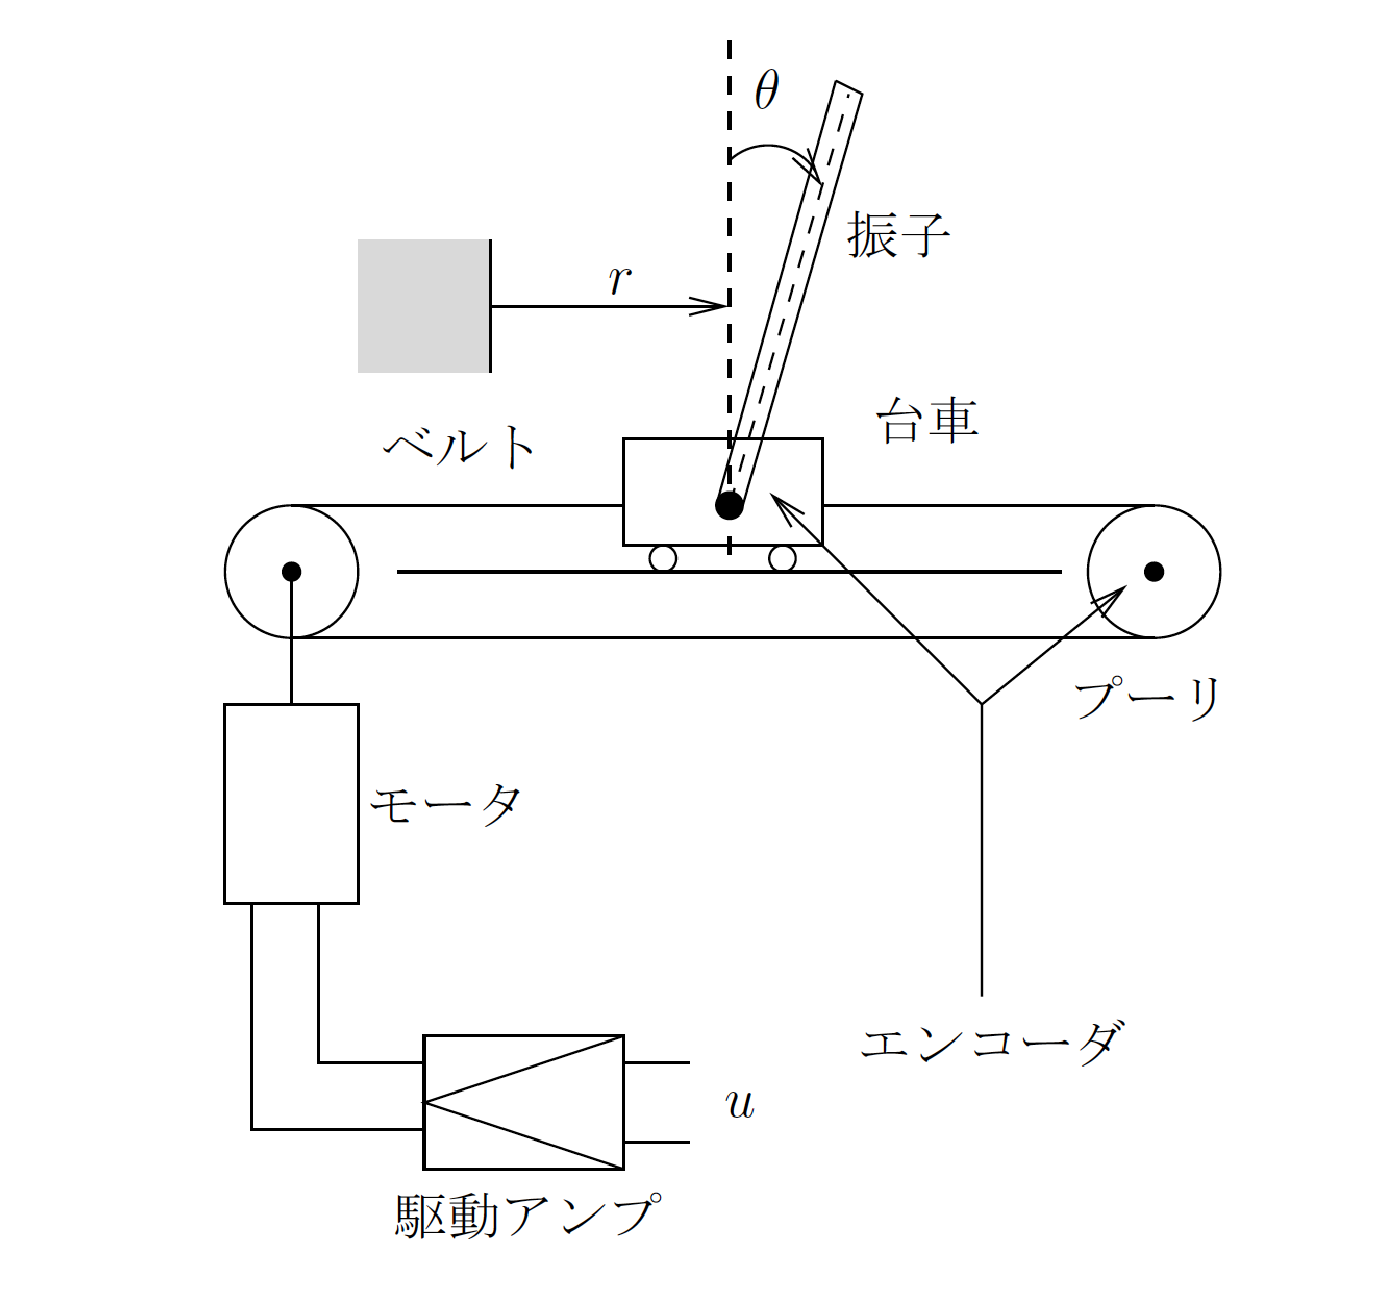
\includegraphics[width=0.6\linewidth]{model.eps}
        \caption{図\ref{pendulum}: 倒立振子系}
        \label{pendulum}
    \end{center}
\end{figure}

図\ref{pendulum}は本実験で使用する倒立振子系である。
系は、モータ、ベルト、プーリ系から成り、台車はモータからの入力によりベルト上を水平方向に動くことができる。
台車の初期状態からの変位を$r$とする。
また、鉛直方向上向きから時計回りを正の方向として、台車に取り付けられた振子が回転した角度を$\theta$とする。
ポテンショメータにより、$r$と$\theta$を測定し、入力$u$を与える。

% =============================== chapter 1 END =============================== %


% ================================= chapter 2 ================================= %
\chapter{モデリング}
\section{数式モデル}
制御器の設計のため、倒立振子系の状態方程式、観測方程式から数式モデルを導出する。

\subsection{状態方程式}

\begin{figure}[htbp]
    \begin{center}
        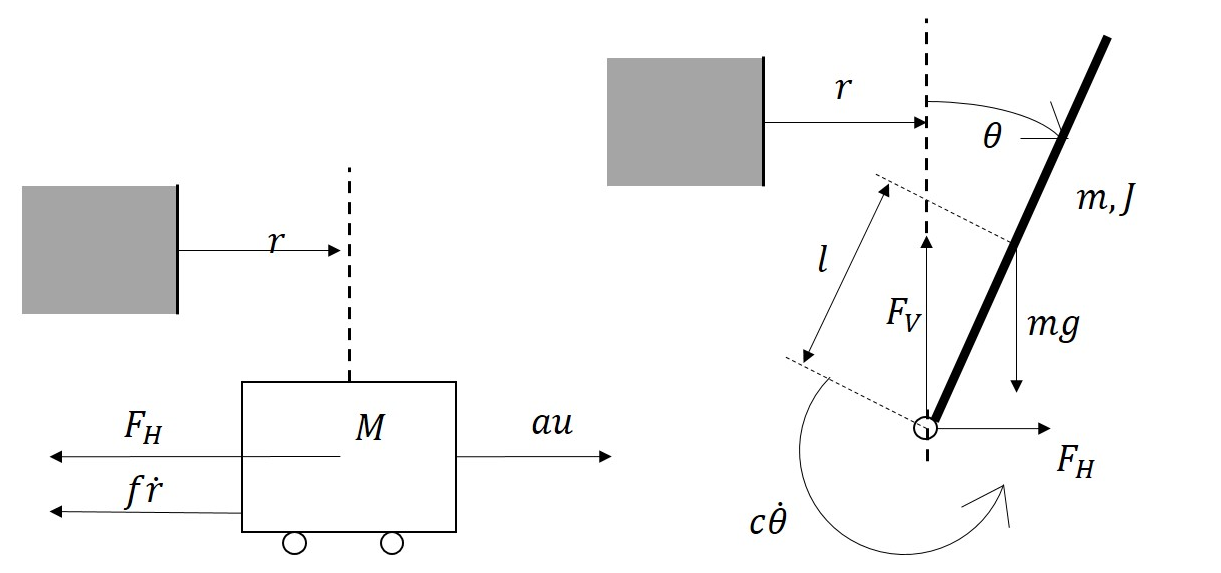
\includegraphics[width=0.6\linewidth]{modeling.eps}
        \caption{図\ref{modeling}: モデリングのための力の分解}
        \label{modeling}
    \end{center}
\end{figure}

図\ref{modeling}から導出した倒立振子系の運動方程式を
式(\ref{modeling:cart1})から式(\ref{modeling:pend2})に示す。

\begin{equation}
    M \ddot r = au - F_{H} - f \dot r
    \label{modeling:cart1}
\end{equation}
\begin{equation}
    J \ddot \theta = lF_{V}\sin \theta - lF_{H}\cos \theta - c \dot \theta
    \label{modeling:pend1}
\end{equation}
\begin{equation}
    m\frac{d^2}{dt^2}(r + l\sin \theta) = F_{H}
    \label{modeling:cart2}
\end{equation}
\begin{equation}
    m\frac{d^2}{dt^2}(l\cos \theta) = F_{V} - mg
    \label{modeling:pend2}
\end{equation}

ただし、$M$,$f$は台車の質量と摩擦係数、$m$,$l$,$c$,$J$は振子の質量、振子の重心から回転軸までの距離、
回転軸摩擦係数、重心周りに働く慣性モーメントである。また、$F_{H}$,$F_{V}$は振子が台車から受ける
水平効力と垂直抗力である。$F$はモータによる台車への駆動力であり、定数$a$、駆動アンプへの入力電圧$u$を用いて
式(\ref{F})で表される。

\begin{equation}
    F = au
    \label{F}
\end{equation}

ここで、系の状態$x$を4つの状態変数からなる縦ベクトルとする。すなわち、
$$
    x = \left [
    \begin{array}{c}
        r \\
        \theta \\
        \dot r \\
        \dot \theta
    \end{array}
    \right ]
$$
と定義する。
次に、式(\ref{modeling:cart1})から式(\ref{modeling:pend2})から倒立振子系の非線形方程式を求める。
式(\ref{modeling:cart1}),式(\ref{modeling:pend1})から$F_{H}$を消去すると、式(\ref{del_Fh})が得られる。

\begin{equation}
    (M + m) \ddot r + (ml\cos \theta) \ddot \theta = au + (ml\sin \theta) \dot \theta^2 - f \dot r
    \label{del_Fh}
\end{equation}

また、式(\ref{modeling:pend1}),式(\ref{modeling:cart2}),式(\ref{modeling:pend2})から
$F_{H}$,$F_{V}$を消去すると、

$$
    J \ddot \theta = l\left(
        m\frac{d^2}{dt^2}\left(
            l\cos \theta + mg
            \right)
        \right)\sin \theta
        -
        l\left(
            m\frac{d^2}{dt^2}\left(
                r + l\sin \theta
            \right)
        \right)\cos \theta
$$

となり、式(\ref{del_Fh_Fv})が得られる。

\begin{equation}
    ml\cos \theta \ddot r + (J + ml^2) \ddot \theta = mgl\sin \theta -c \dot \theta
    \label{del_Fh_Fv}
\end{equation}

式(\ref{del_Fh}),式(\ref{del_Fh_Fv})を行列表現すると、

$$
    % --- left side --- %
    % --- first matrix --- %
    \left[
    \begin{array}{cc}
        M + m          &  ml\cos \theta \\
        ml\cos \theta  &  J + ml^2
    \end{array}
    \right]
    % --- second matrix --- %
    \left[
    \begin{array}{c}
        \ddot r \\
        \ddot \theta
    \end{array}    
    \right]
    =
    % --- right side --- %
    \left[
        \begin{array}{c}
            -f \dot r + ml(\sin \theta) \dot \theta^2 + au \\
            mgl\sin \theta - c \dot \theta
        \end{array}
    \right]
$$

$$
    % --- left side --- %
    \left[
    \begin{array}{c}
        \ddot r \\
        \ddot \theta
    \end{array}    
    \right]
    =
    % --- right side --- %
    % --- first matrix --- %
    \left[
    \begin{array}{cc}
        M + m          &  ml\cos \theta \\
        ml\cos \theta  &  J + ml^2
    \end{array}
    \right]^{-1}
    % --- second matrix --- %
    \left[
        \begin{array}{c}
            -f \dot r + ml(\sin \theta) \dot \theta^2 + au \\
            mgl\sin \theta - c \dot \theta
        \end{array}
    \right]
$$

となる。よって、

\begin{equation}
    \dot x = f(x, u) = 
    \left[
        \begin{array}{c}
            \dot r \\
            \dot \theta \\
            K^{-1}
            \left[
                \begin{array}{c}
                    -f \dot r + ml(\sin \theta) \dot \theta^2 + au \\
                    mgl\sin \theta - c \dot \theta
                \end{array}
            \right]
        \end{array}    
    \right],\
    K = 
    \left[
        \begin{array}{cc}
            M + m          &  ml\cos \theta \\
            ml\cos \theta  &  J + ml^2
        \end{array}
    \right]
    \label{nonlinear}
\end{equation}

が得られる。本実験では、不安定平衡点$x=0$近傍で線形化したモデルを採用できる。
$\theta$に関して式(\ref{nonlinear})を一次近似すると、
$\sin \theta \approx \theta,\ \cos \theta \approx 1,\ \theta^2 \approx 0$と近似できることから、

\begin{equation}
% --- Matrix x_dot --- %
    \dot x = 
    \left[
        \begin{array}{c}
            \dot r \\
            \dot \theta \\
            K^{-1}
            \left[
                \begin{array}{c}
                    -f \dot r + au \\
                    mgl \theta - c \dot \theta
                \end{array}
            \right]
        \end{array}    
    \right],\
    %--- Matrix K ---%
    K = 
    \left[
        \begin{array}{cc}
            M + m  &  ml \\
            ml     &  J + ml^2
        \end{array}
    \right]
\end{equation}

を得る。線形化された倒立振子系の状態方程式は、式(\ref{linear_general})のように表現される。

\begin{equation}
    \dot x = Ax + Bu
    \label{linear_general}
\end{equation}

ここで、

$$
    % --- Matrix A --- %
    A = 
    \left[
        \begin{array}{cc}
            O_{2 \times 2}  &  I_{2} \\
            A_{21}          &  A_{22}
        \end{array}
    \right],\
    % --- Matrix B --- %
    B = 
     \left[
        \begin{array}{c}
            O_{2 \times 1} \\
            B_{2}
        \end{array}
    \right]
$$

である。ただし、

$$
    A_{21} = K^{-1}
    \left[
        \begin{array}{cc}
            0  &  0 \\
            0  &  mgl
        \end{array}    
    \right],\
    A_{22} = K^{-1}
    \left[
        \begin{array}{cc}
            -f  &  0 \\
            0   &  -c
        \end{array}    
    \right],\
    B_{2} = K^{-1}
    \left[
        \begin{array}{c}
            a \\
            0
        \end{array}    
    \right]
$$

である。

\subsection{観測方程式}
2つの観測出力は、

$$
    y_{1} = c_{1} r
$$

$$
    y_{2} = c_{2} \theta
$$

のように表される。ここで、$c_{1}$は変位・電圧変換係数, $c_{2}$は角度・電圧変換係数である。
これらからなる縦ベクトル、すなわち出力$y$を、

$$
    y = 
    \left[
        \begin{array}{c}
            y_{1} \\
            y_{2}
        \end{array}    
    \right]
$$

と定義すると、倒立振子系に対する観測方程式を、

\begin{equation}
    y = Cx
\end{equation}

と表せる。ただし、

$$
    % --- Matrix N --- %
    N = 
    \left[
        \begin{array}{cc}
            c_{1}  &  0 \\
            0      &  C_{2}
        \end{array}
    \right],\
    % --- Matrix C --- %
    C = 
    \left[
        \begin{array}{cc}
            N  &  O_{2 \times 2}
        \end{array}
    \right]
    =
    \left[
        \begin{array}{cccc}
            c_{1}  &    0    &    0    &    0 \\
            0      &  c_{2}  &    0    &    0
        \end{array}
    \right]
$$

である。

% =============================== chapter 2 END =============================== %

% ================================= chapter 3 ================================= %
\chapter{制御系設計}



% =============================== chapter 3 END =============================== %

% ================================= chapter 4 ================================= %
\chapter{シミュレーション}


% =============================== chapter 4 END =============================== %

% ================================= chapter 5 ================================= %
\chapter{実験}


% =============================== chapter 5 END =============================== %

% ================================= chapter 6 ================================= %
\chapter{おわりに}


% =============================== chapter 6 END =============================== %



% --- main END ---%
\end{document}
